\documentclass[a4paper,12pt,abstracton,titlepage]{scrartcl}

\usepackage[ngerman]{babel}
\usepackage[T1]{fontenc}
\usepackage[utf8]{inputenc} % Umlaute, evtl. vom Betriebssystem abhaengig
\usepackage{lmodern}
\usepackage{pgfgantt}
\usepackage{titlesec}
\usepackage{float}
\usepackage{floatflt}
\usepackage{blindtext}
\usepackage{amsmath}
\usepackage{tabularx,url}


\titleformat*{\section}{\large\bfseries}
\titleformat*{\subsection}{\large\bfseries}
\titleformat*{\subsubsection}{\large\bfseries}
\titleformat*{\paragraph}{\large\bfseries}
\titleformat*{\subparagraph}{\large\bfseries}

\renewcaptionname{ngerman}{\figurename}{Abb.}

%\titlehead{Ulm University}
%\title{Title}
%\subject{Subject}
%\author{Author}
%\publishers{%
	%\rule{\textwidth}{0.4pt} \\
	%\vspace{0.5cm}
    %\normalfont\normalsize%
    %\parbox{0.9\linewidth}{%
    %    Abstract or Introduction
    %} \\
    %\vspace{0.5cm}
   	%\rule{\textwidth}{0.4pt}
%}

\begin{document}
%\maketitle

%%% begin costom title
{\Large\noindent \emph{ESIEE Paris}}

{\Large\noindent \emph{IGI-3008}}
\begin{center}
	{\large Cryptographie	 \\ \large Léa MENERET, Fathima SAHADATTALY, Ulrike KULZER \\ \today}
\end{center}
%%% end custom title

\setcounter{page}{1} % reset page counter to one for the first page, leave the title page out

\section{Contexte}
\subsection{En général}
La cryptographie est une technique utilisée pour rendre incompréhensible à autrui un message entre un expéditeur et un destinataire. Ce procédé a notamment été utilisé en période de guerre pour permettre des attaques surprises. 
Le principe est le suivant : L'expéditeur à partir d'une clé crypte son message et l'envoie au destinataire. Celui-ci possède aussi la clé qui va lui permettre ainsi de décrypter le message.

\subsection{Histoire}
La cryptographie est utilisée depuis l'Antiquité mais certaines de ces méthodes les plus abouties datent du 20e siècle. Il existe différents principes de cryptage plus ou moins compliqués tels que le chiffre de César, le chiffre de Vigenère et celui de la machine Enigma.

\subsubsection{Le chiffre de César :}
\begin{floatingfigure}[r]{8.3cm}
	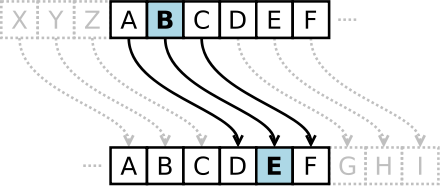
\includegraphics[width=0.5\textwidth]{./Pictures/chiffreCesar.png}
	%\caption{principe du chiffre de César}
	\label{cesar}
\end{floatingfigure}
Ce procédé a été inventé lors de l'époque romaine par Jules César pour ses communications secrètes. En décalant l'alphabet par un entier donné chaque lettre est associée à une nouvelle lettre, ainsi on peut crypter le message initiale en remplaçant chaque lettre par la nouvelle lettre attribuée.

\newpage
\subsubsection{Le chiffre de Vigenère :}
\begin{floatingfigure}[r]{8.3cm}
	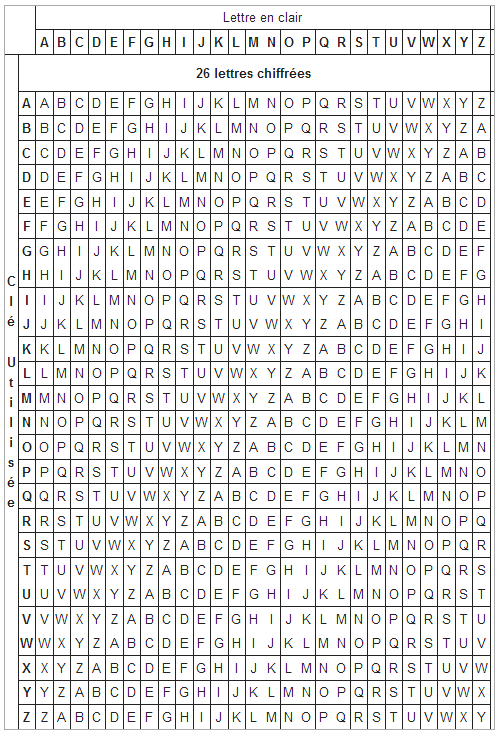
\includegraphics[width=0.5\textwidth]{./Pictures/tableauVigenere.png}
	%\caption{tableau de Vigenère}
	\label{vigenere}
\end{floatingfigure}
Il a été inventé au 16e siècle par Blaise de Vigenère et est basé sur le tableau à droite. Une clé (un mot) est répétée et mis sous le message et de cette manière on peut trouver les lettres correspondantes à partir du tableau.\\
Exemple:
Clé : musique\\
Texte : J'adore écouter la radio toute la journée.\\
Texte en claire et en dessous la clé répétée:\\
j'adore ecouter la radio\\
M USIQU EMUSIQU EM USIQU\\
\textasciicircum\ \ \\textasciicircum\textasciicircum\textasciicircum\\
| ||Colonne O, ligne I : on obtient la lettre W.\\
| |Colonne D, ligne S : on obtient la lettre V.\\
| Colonne A, ligne U : on obtient la lettre U.\\
Colonne J, ligne M : on obtient la lettre V.%\footnote{https://fr.wikipedia.org/wiki/Chiffre_de_Vigen\%C3\%A8re}

\subsubsection{La machine Enigma :}
L’Enigma est une machine de cryptographie inventée par Arthur Scherbius en 1919. Elle a été utilisée durant la Seconde Guerre mondiale pour la communication secrète entre les différentes unités de l’armée allemande.
La machine est constituée de cinq rotors dont un réflecteur, d’un clavier, d’un tableau de permutation et de lampes pour chaque lettre. Pour l’allumer il faut une batterie de 4,5 Volt.
Le principe est simple : Lorsqu’on appuie sur une lettre du clavier, un courant électrique va être envoyé au tableau de permutation dans lequel la lettre entrée est échangée avec une autre lettre si elles sont connectées. Puis il passera la première fois par les quatre rotors : Dans chacun des trois rotors au milieu il y a un décalage des lettres qui s’opère. À la fin les lettres sont permutées encore une fois dans le réflecteur qui les renvoie par les rotors au tableau de permutation ce qui permettra à une lampe correspondant à une lettre de s’allumer. Ainsi pour chaque lettre on relève la lettre codée, on obtient alors notre message crypté.

\section{Fonctionnalité}
\subsection{Différents états du programme}
\begin{figure}[tpbh]
	\centering
  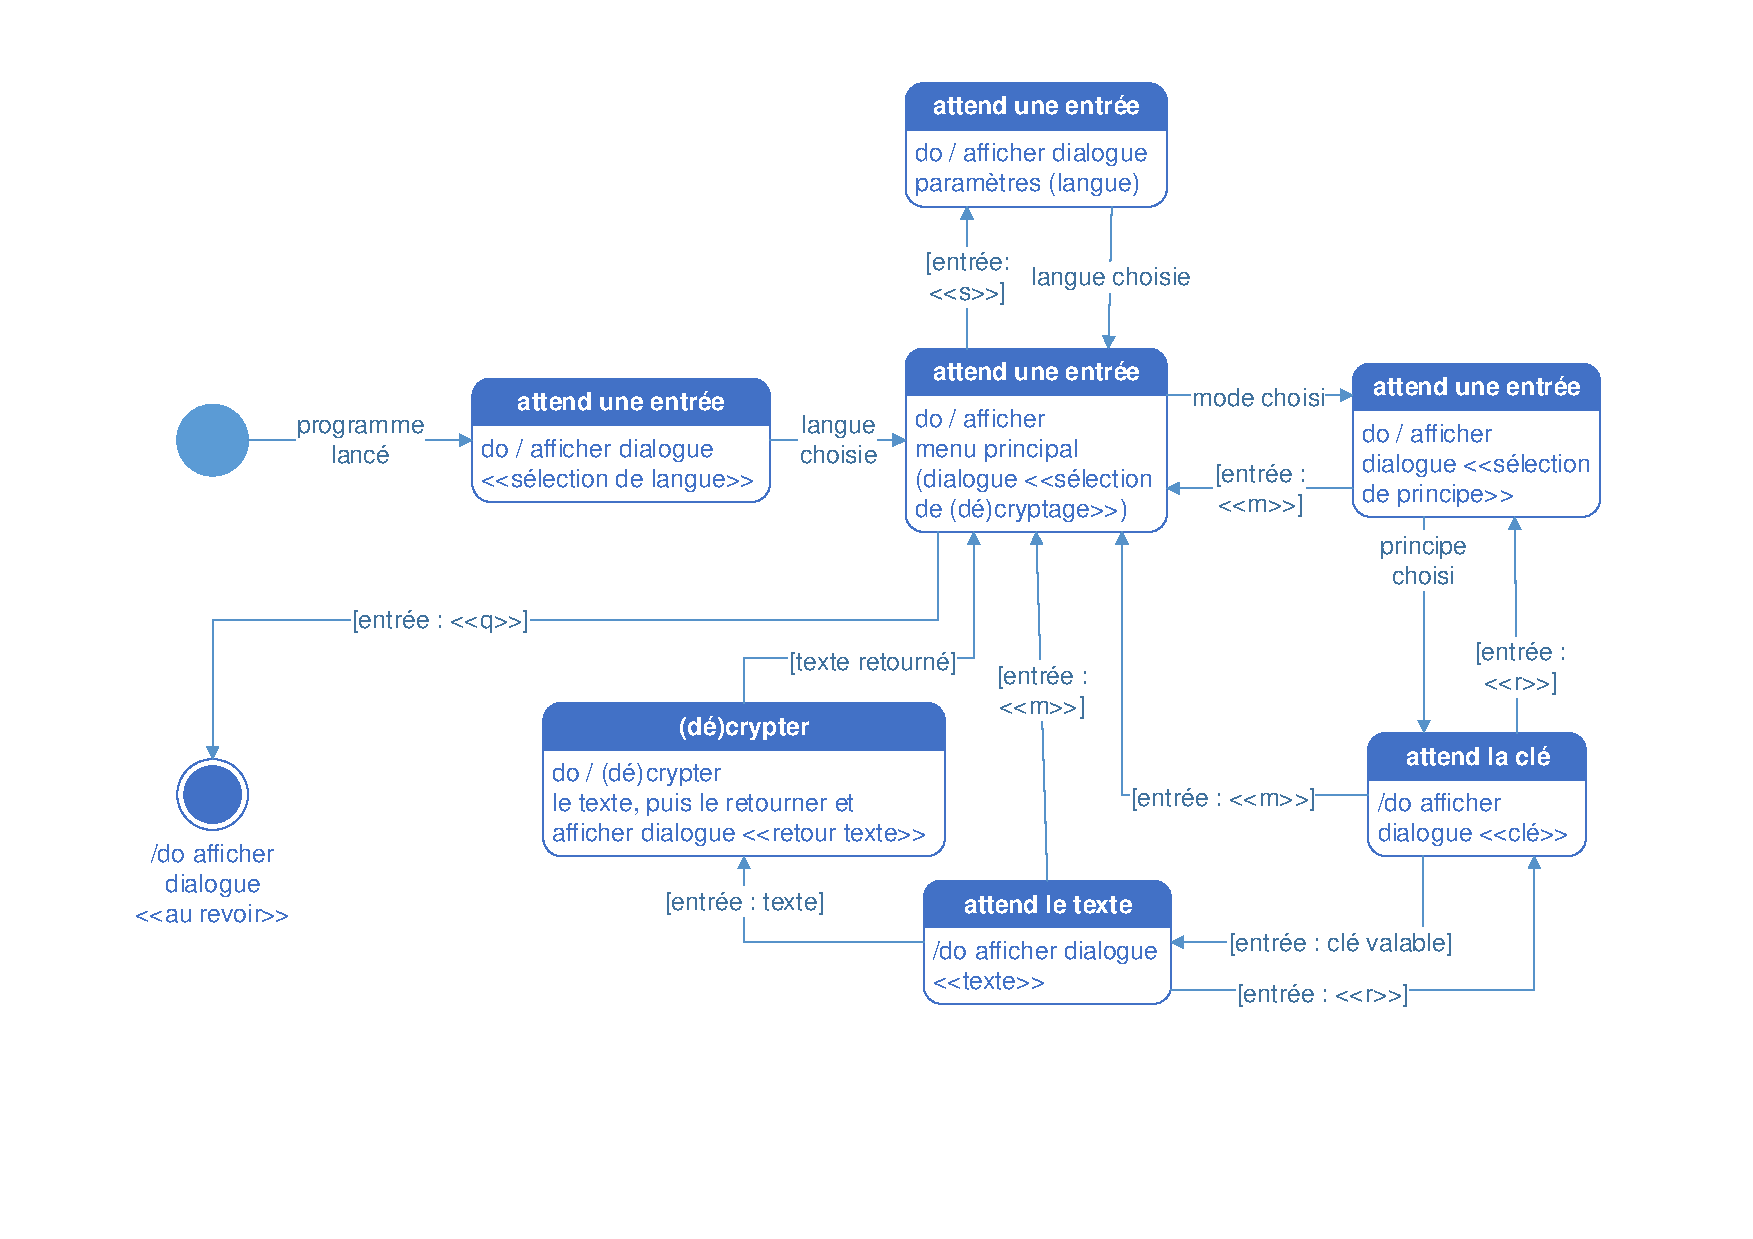
\includegraphics[width=\textwidth, trim=25mm 10mm 10mm 8mm, clip]{./Diagrammes/diagrammeDesEtats.pdf}
  %\caption{Différents états du programme}
	\label{img:etats}
\end{figure}

\subsection{En général}
\blindtext

\subsection{En détail et coupé en modules}
\blindtext


\section{Interfaces utilisateurs}
\blindtext




% (CIE\footnote{CIE = Commission internationale de l’éclairage})  "`Inviwo"'\footnote{Interactive Visualization Workshop}

%\section{Grundlagen}
\begin{floatingfigure}[r]{6cm}
%	\includegraphics[width=0.3\textwidth]{./Bilder/1cie.png}
	\caption{CIE"=Normvalenzsystem}
	\label{cie}
\end{floatingfigure}

%(meist im CIE"=Normvalenzsystem) oder verschiedenen Farbkörpern, z. B. Würfel oder Kegeln, dargestellt. Als Beispiel sieht man in Abbildung \ref{cie} eine Darstellung des Standard"=RGB"=Farbraums


\begin{floatingfigure}[l]{5.3cm}
%	\includegraphics[width=0.25\textwidth]{./Bilder/2venn.png}
	\caption{Prinzip der additiven Farbmischung}
	\label{venn}
\end{floatingfigure}

\par

% wodurch weißes Licht reflektiert wird (s. Abb. \ref{venn}). 


\vspace{2em}
%\section{Farbmodell, Konvertierung und Implementierung}
%\subsection{Vorstellung der Farbmodelle}
%\subsubsection{Das Farbmodell RGB} 
%(für Genaueres siehe \cite{kompendium}).

\subsubsection{Das Farbmodell HSV}
\begin{floatingfigure}[r]{8.3cm}
	%\includegraphics[width=0.5\textwidth]{./Bilder/hsvKegel.png}
	\caption{HSV-Farbkörper}
	\label{hsv}
\end{floatingfigure} 


\vspace{1em}
\subsubsection{Die Farbmodelle YUV, YPbPr und YCbCr}
% NTSC\footnote{für Details siehe \cite{linkfangNTSC}} und des PAL-Verfahrens\footnote{für Details siehe \cite{linkfangPAL}} entwickelt und basiert auf dem RGB"= Farbmodell. 



\begin{figure}[htbp]
\begin{minipage}[t]{0.48\textwidth}
  \begin{center}
    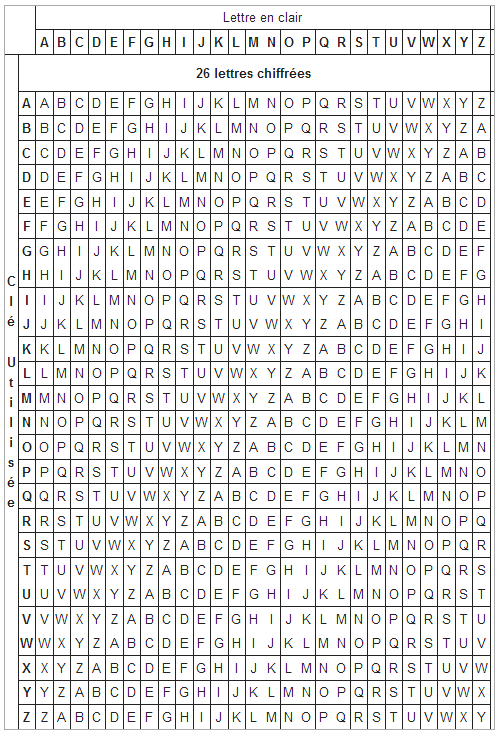
\includegraphics[height=5.6cm]{./Pictures/tableauVigenere.png}
    \caption{Originalbild}
    \label{originalScot}
  \end{center}
\end{minipage}
\begin{minipage}[t]{0.52\textwidth}
  \begin{center}
    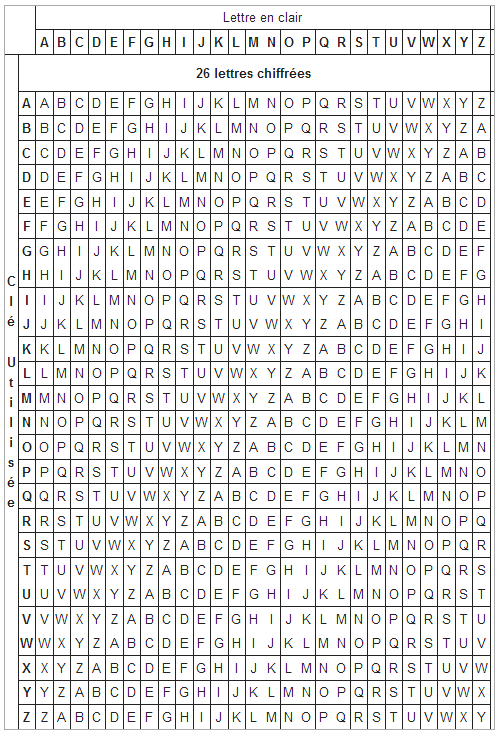
\includegraphics[height=5.6cm]{./Pictures/tableauVigenere.png}
    \caption{Bild nach der Konvertierung}
    \label{rgb2hsv}
  \end{center}
\end{minipage}
\end{figure}


 

\begin{figure}[htbp]
\begin{minipage}[t]{0.48\textwidth}
  \begin{center}
   % \includegraphics[height=5.6cm]{./Bilder/bilderKonv/original/canvas_rgb2hsv_cut.png}
    \caption{Bild im HSV"=Farbraum}
    \label{hsvVorher}
  \end{center}
\end{minipage}
\begin{minipage}[t]{0.52\textwidth}
  \begin{center}
   % \includegraphics[height=5.6cm]{./Bilder/bilderKonv/original/canvas_hsv2rgb_cut.png}
    \caption{Bild nach der Konvertierung}
    \label{hsv2rgb}
  \end{center}
\end{minipage}
\end{figure}

% "`Standard Definition Television"', HDTV für "`High Definition Television'".

\newpage
\begin{figure}[htbp]
\begin{minipage}[t]{0.48\textwidth}
  \begin{center}
    %\includegraphics[height=5cm]{./Bilder/bilderKonv/balloons_fehlerhaft/rgb2hsv_cut.png}
    \caption{RGB nach HSV}
    \label{errorBall}
    \begin{small}
    Quelle: w.hsv
    \end{small}
  \end{center}
\end{minipage}
\begin{minipage}[t]{0.48\textwidth}
  \begin{center}
    %\includegraphics[height=5cm]{./Bilder/bilderKonv/balloons_fehlerhaft/testGes.png}
    \caption{HSV nach RGB mit vergrößertem Ausschnitt}
    \label{errorBallRGB}
  \end{center}
\end{minipage}
\end{figure}



\section{Referenzen}
\nocite{*} 
%\renewcommand{\bibname}{\section{Sources}} % Redefine bibname
\bibliographystyle{IEEEtran} % Set any options you want
\bibliography{bibliography} % Build the bibliography

\subsection*{Bildquellen}

\begin{tabularx}{0.95\linewidth}{@{}>{\bfseries}l@{\hspace{0.5em}}X@{}}
    Abb. \ref{cie}   &     \url{http://www.itwissen.info/definition/lexikon/Standard-RGB-sRGB-standard-RGB.html} (31.01.2017)
    \\
    Abb. \ref{venn}   &	   \url{https://www.saxoprint.de/blog/der-farbraum-rgb-und-cmyk-im-vergleich/} (31.01.2017)
    \\
    Abb. \ref{hsv}   &     \url{http://de.mathworks.com/help/images/convert-from-hsv-to-rgb-color-space.html?requestedDomain=www.mathworks.com} (07.02.2017)
    \\
    Abb. \ref{originalScot}   &     Ulrike Kulzer
    \\
    Abb. \ref{errorBall}   &     Originalbild:
    \url{https://www.tutorialspoint.com/java_dip/color_space_conversion.htm} (08.02.2017)
    \\
\end{tabularx}



\begin{tabular}[t]{lr}
Naher Osten & 65\%\\
Lateinamerika & 13\%\\
\end{tabular}\\

%\begin{itemize}
%\item \blindtext
%\item \blindtext
%\end{itemize}
%\begin{enumerate}
%\item \blindtext
%\item \blindtext
%\end{enumerate}
%\begin{description}
%\item [Ant] \blindtext
%\item [Elephant] \blindtext

%\textbf{greatest} 
%\underline{science} 
%\textbf{\textit{accident}}.


\end{document}




% LABEL UNTER CAPTION

